\documentclass[11pt]{article}
\usepackage{certmachine}
\usepackage{graphicx}
\usepackage{float}
\graphicspath{{fig/}}
%% generated by tools/paper-numbers/mfg-multiplicity.js from certs/mfg-regime-map.json, certs/mfg2p-regime-map.json, certs/mfg-cap-multiplicity.json, certs/mfg-cap-census-N*-c-12.json, certs/monoflow-spectrum.json, certs/frontier-measurement.json and the live batteries — do not edit (git 054078d19462)
\newcommand{\RepoCommit}{054078d19462}
\newcommand{\OneGenerated}{2026-08-28}
\newcommand{\OneCommitDate}{2026-08-28}
\newcommand{\OneSigma}{0.5}
\newcommand{\OneN}{16}
\newcommand{\OneNu}{1.02}
\newcommand{\OneCLo}{-18}
\newcommand{\OneCHi}{2}
\newcommand{\OneALo}{0}
\newcommand{\OneAHi}{1.2}
\newcommand{\OneBaseC}{0.125}
\newcommand{\OneBaseA}{0.05}
\newcommand{\OneMaxDepth}{2}
\newcommand{\OneCollapseTol}{0.05}
\newcommand{\OneCellCap}{40{,}000}
\newcommand{\OneSeconds}{2{,}037}
\newcommand{\OneSecondsMin}{34}
\newcommand{\OneCStar}{-9.8696}
\newcommand{\OneCStarSix}{-9.869604}
\newcommand{\OneCells}{19{,}800}
\newcommand{\OneMult}{11{,}330}
\newcommand{\OneUniq}{384}
\newcommand{\OneUnd}{8{,}086}
\newcommand{\OneUndEnclosed}{6{,}470}
\newcommand{\OneUndNothing}{1{,}616}
\newcommand{\OneDomainArea}{24}
\newcommand{\OneMultArea}{7.372}
\newcommand{\OneUniqArea}{2.400}
\newcommand{\OneUndArea}{14.228}
\newcommand{\OneMultPct}{30.7\%}
\newcommand{\OneUniqPct}{10.0\%}
\newcommand{\OneUndPct}{59.3\%}
\newcommand{\OneUndEncArea}{13.597}
\newcommand{\OneUndEncPct}{56.7\%}
\newcommand{\OneFinestC}{0.03125}
\newcommand{\OneFinestA}{0.0125}
\newcommand{\OneRasterC}{640}
\newcommand{\OneRasterA}{96}
\newcommand{\OneDepthRows}{0 & 0.125 $\times$ 0.05 & 1{,}973 & 0 & 384 & 1{,}589 \\
1 & 0.0625 $\times$ 0.025 & 4{,}015 & 2{,}514 & 0 & 1{,}501 \\
2 & 0.03125 $\times$ 0.0125 & 13{,}812 & 8{,}816 & 0 & 4{,}996 \\}
\newcommand{\OneMultWidthText}{2{,}514 at width 0.0625 and 8{,}816 at width 0.03125}
\newcommand{\OneMultWidthWide}{0.0625}
\newcommand{\OneMultWidthWideCount}{2{,}514}
\newcommand{\OneMultWidthFine}{0.03125}
\newcommand{\OneMultWidthFineCount}{8{,}816}
\newcommand{\OneWorstSepRatio}{289.5}
\newcommand{\OneBestSepRatio}{$1.6\times10^{4}$}
\newcommand{\OneMinDensity}{$2.80\times10^{-7}$}
\newcommand{\OneWorstKappa}{0.9956}
\newcommand{\OneMaxRadius}{$2.89\times10^{-2}$}
\newcommand{\OneMultCMin}{-18}
\newcommand{\OneMultCMax}{-10.84375}
\newcommand{\OneMultAMin}{0}
\newcommand{\OneMultAMax}{1.2}
\newcommand{\OneUniqCMin}{0}
\newcommand{\OneUniqCMax}{2}
\newcommand{\OneMinDensityC}{[-16.3125,\ -16.25]}
\newcommand{\OneMinDensityA}{[0.3,\ 0.325]}
\newcommand{\OneTightC}{[-11.3125,\ -11.28125]}
\newcommand{\OneTightA}{[0.225,\ 0.2375]}
\newcommand{\OneTightDepth}{2}
\newcommand{\OneTightRAligned}{$2.039\times10^{-3}$}
\newcommand{\OneTightRHerding}{$1.890\times10^{-2}$}
\newcommand{\OneTightKappaAligned}{0.2777}
\newcommand{\OneTightKappaHerding}{0.9759}
\newcommand{\OneTightZoneAligned}{0.2233}
\newcommand{\OneTightZoneHerding}{0.3415}
\newcommand{\OneTightYzeroAligned}{$1.46\times10^{-3}$}
\newcommand{\OneTightYzeroHerding}{$6.42\times10^{-3}$}
\newcommand{\OneTightZtwoAligned}{26.69}
\newcommand{\OneTightZtwoHerding}{33.58}
\newcommand{\OneTightSep}{6.0626}
\newcommand{\OneTightRSum}{$2.094\times10^{-2}$}
\newcommand{\OneTightRatio}{289.5}
\newcommand{\OneTightMinM}{0.2529}
\newcommand{\OneTightBoneAligned}{[0.0793,\ 0.0860]}
\newcommand{\OneTightBoneHerding}{[0.4461,\ 0.4537]}
\newcommand{\OneReasonRows}{5{,}470 & only one solution found at the cell midpoint: a second branch is not excluded, it is not exhibited \\
1{,}127 & aligned branch: discriminant $\le 0$, no radius closes the contraction over the box \\
999 & herding branch: discriminant $\le 0$, no radius closes the contraction over the box \\
489 & aligned branch: $Z_1 \ge 1$ over the box, the midpoint inverse does not control the whole cell \\
1 & herding branch: $\kappa = Z_1 + Z_2 r \ge 1$ at the smallest admissible radius (a self-map, not a contraction) \\}
\newcommand{\OneWhyOnlyOne}{5{,}470}
\newcommand{\OneWhyZone}{489}
\newcommand{\OneWhyDisc}{2{,}126}
\newcommand{\TwoCommitDate}{2026-08-29}
\newcommand{\TwoSigma}{0.5}
\newcommand{\TwoCs}{1}
\newcommand{\TwoA}{1}
\newcommand{\TwoN}{16}
\newcommand{\TwoNu}{1.02}
\newcommand{\TwoSLo}{0}
\newcommand{\TwoSHi}{15}
\newcommand{\TwoDLo}{0}
\newcommand{\TwoDHi}{1.5}
\newcommand{\TwoSFine}{10}
\newcommand{\TwoBaseS}{0.2}
\newcommand{\TwoBaseD}{0.25}
\newcommand{\TwoFineS}{0.025}
\newcommand{\TwoFineD}{0.025}
\newcommand{\TwoMaxDepth}{1}
\newcommand{\TwoCollapseTol}{$1\times10^{-4}$}
\newcommand{\TwoCellCap}{60{,}000}
\newcommand{\TwoAtlasSeg}{2{,}573}
\newcommand{\TwoCells}{21{,}567}
\newcommand{\TwoMult}{11{,}628}
\newcommand{\TwoUniq}{24}
\newcommand{\TwoUnd}{9{,}915}
\newcommand{\TwoUndEnclosed}{5{,}285}
\newcommand{\TwoUndNothing}{4{,}630}
\newcommand{\TwoDomainArea}{22.5}
\newcommand{\TwoMultArea}{5.465}
\newcommand{\TwoUniqArea}{1.200}
\newcommand{\TwoUndArea}{15.835}
\newcommand{\TwoMultPct}{24.3\%}
\newcommand{\TwoUniqPct}{5.3\%}
\newcommand{\TwoUndPct}{70.4\%}
\newcommand{\TwoFinestS}{0.0125}
\newcommand{\TwoFinestD}{0.0125}
\newcommand{\TwoRasterS}{1{,}200}
\newcommand{\TwoRasterD}{120}
\newcommand{\TwoSizeRows}{0.2 $\times$ 0.25 & 264 \\
0.1 $\times$ 0.125 & 144 \\
0.025 $\times$ 0.025 & 8{,}947 \\
0.0125 $\times$ 0.0125 & 12{,}212 \\}
\newcommand{\TwoWorstSepRatio}{246.2}
\newcommand{\TwoBestSepRatio}{7{,}957}
\newcommand{\TwoMinDensity}{0.1715}
\newcommand{\TwoWorstKappa}{0.9976}
\newcommand{\TwoMultSmin}{11.2375}
\newcommand{\TwoMultSmax}{15}
\newcommand{\TwoMultDmax}{1.5}
\newcommand{\TwoGap}{11.23}
\newcommand{\TwoMultUnreach}{11{,}463}
\newcommand{\TwoMultUnreachPct}{98.6\%}
\newcommand{\TwoMultUnreachAreaPct}{23.9\%}
\newcommand{\TwoUniqSmax}{0.8}
\newcommand{\TwoUniqDetMin}{0.577}
\newcommand{\TwoUniqRMax}{$1.15\times10^{-3}$}
\newcommand{\TwoUniqKappaMax}{0.1172}
\newcommand{\TwoUniqMinM}{0.8977}
\newcommand{\TwoFirstS}{[11.2375,\ 11.25]}
\newcommand{\TwoFirstD}{[0.475,\ 0.4875]}
\newcommand{\TwoFirstRatio}{248.4}
\newcommand{\TwoTightS}{[11.2375,\ 11.25]}
\newcommand{\TwoTightD}{[0.525,\ 0.5375]}
\newcommand{\TwoTightRPrimary}{$6.421\times10^{-3}$}
\newcommand{\TwoTightRSegregated}{$1.252\times10^{-2}$}
\newcommand{\TwoTightKappaPrimary}{0.8808}
\newcommand{\TwoTightKappaSegregated}{0.8914}
\newcommand{\TwoTightSep}{4.6643}
\newcommand{\TwoTightNeed}{$1.894\times10^{-2}$}
\newcommand{\TwoTightRatio}{246.2}
\newcommand{\TwoTightMinM}{0.5993}
\newcommand{\TwoReasonRows}{5{,}285 & one equilibrium enclosed over the cell; the monotonicity hypothesis fails somewhere in it, so uniqueness is not available (not refinable) \\
2{,}151 & primary branch: discriminant $\le 0$ \\
168 & primary branch: $Z_1 \ge 1$ over the box \\
1 & primary branch: $\kappa \ge 1$ at the smallest admissible radius \\
1{,}623 & segregated branch: discriminant $\le 0$ \\
105 & segregated branch: $Z_1 \ge 1$ over the box \\
4 & segregated branch: $\kappa \ge 1$ at the smallest admissible radius \\
1 & segregated branch: no radius verified $p(r) < 0$ \\
577 & both branches refused, each with a named mode \\}
\newcommand{\TwoWhyMonotone}{5{,}285}
\newcommand{\TwoWhyMonotoneNoRef}{4{,}191}
\newcommand{\TwoWhyMonotoneRef}{1{,}094}
\newcommand{\MultDate}{2026-09-02}
\newcommand{\MultSigma}{0.5}
\newcommand{\MultNu}{1.02}
\newcommand{\MultRows}{-11 & 16 & $7.05\times10^{-15}$ & $4.73\times10^{-13}$ & 0.273 & 6.701 & $9.46\times10^{-13}$ & $2.97\times10^{-1}$ \\
-12 & 16 & $7.22\times10^{-15}$ & $1.63\times10^{-11}$ & 0.321 & 10.786 & $3.26\times10^{-11}$ & $1.62\times10^{-1}$ \\
-14 & 16 & $7.23\times10^{-15}$ & $5.90\times10^{-9}$ & 0.409 & 16.760 & $1.18\times10^{-8}$ & $5.63\times10^{-2}$ \\
-16 & 16 & $1.34\times10^{-14}$ & $2.14\times10^{-7}$ & 0.495 & 21.433 & $4.28\times10^{-7}$ & $1.90\times10^{-2}$ \\
-20 & 24 & $1.51\times10^{-14}$ & $9.27\times10^{-9}$ & 0.441 & 30.516 & $1.86\times10^{-8}$ & $3.28\times10^{-3}$ \\
-24 & 32 & $1.46\times10^{-14}$ & $1.09\times10^{-9}$ & 0.415 & 39.850 & $2.18\times10^{-9}$ & $4.44\times10^{-4}$ \\}
\newcommand{\MultCount}{6}
\newcommand{\MultCouplings}{-11,\ -12,\ -14,\ -16,\ -20,\ -24}
\newcommand{\MultCouplingsText}{$-11$, $-12$, $-14$, $-16$, $-20$, $-24$}
\newcommand{\MultCMin}{-11}
\newcommand{\MultCMax}{-24}
\newcommand{\MultMinM}{$4.44\times10^{-4}$}
\newcommand{\MultMaxKappa}{0.495}
\newcommand{\MultBoundaryC}{-9.5}
\newcommand{\CensusRows}{2 & 5 & 3 & 2{,}077 & 86 & 0.08 \\
3 & 7 & 3 & 21{,}642 & 263 & 0.76 \\
4 & 9 & 3 & 335{,}862 & 1{,}843 & 18 \\
5 & 11 & 3 & 6{,}954{,}073 & 22{,}036 & 587 \\}
\newcommand{\CensusDate}{2026-09-01}
\newcommand{\CensusBoxesFive}{6{,}954{,}073}
\newcommand{\CensusSecondsFive}{10}
\newcommand{\CensusSplit}{0.537}
\newcommand{\MonoCommitDate}{2026-09-06}
\newcommand{\MonoInstances}{7}
\newcommand{\MonoDecided}{5}
\newcommand{\MonoUndecided}{2}
\newcommand{\MonoDecidedIds}{C1, M1, M2, H1, H2}
\newcommand{\MonoUndecidedIds}{R1 and H0}
\newcommand{\MonoRows}{C1 & (0.5, 1, 0) & aligned & 16 & not a gradient & $[-20.240,\ -20.239] + i\,[4.414,\ 4.415]$ & $1.1\times10^{-13}$ & $5.9\times10^{-16}$ \\
M1 & (0.5, 1, 1) & aligned & 16 & not a gradient & $[-20.262,\ -20.261] + i\,[4.598,\ 4.599]$ & $1.1\times10^{-13}$ & $1.6\times10^{-15}$ \\
M2 & (0.5, 1, 0.5) & aligned & 16 & not a gradient & $[-20.245,\ -20.244] + i\,[4.461,\ 4.462]$ & $1.1\times10^{-13}$ & $1.2\times10^{-15}$ \\
R1 & (0.3, 2, 1.5) & aligned & 20 & not decided & 7 real eigenvalues reached (floats) & $2.0\times10^{-13}$ & $5.6\times10^{-15}$ \\
H1 & (0.5, -12, 0) & herding & 16 & not a gradient & $[-17.134,\ -17.133] + i\,[17.965,\ 17.966]$ & $2.0\times10^{-12}$ & $1.7\times10^{-11}$ \\
H2 & (0.5, -12, 0.5) & herding & 16 & not a gradient & $[-19.796,\ -19.795] + i\,[17.038,\ 17.039]$ & $1.9\times10^{-12}$ & $4.4\times10^{-12}$ \\
H0 & (0.5, -12, 0) & aligned & 16 & not decided & 6 real eigenvalues reached (floats) & $1.3\times10^{-12}$ & $7.3\times10^{-15}$ \\}
\newcommand{\MonoImMin}{4.41}
\newcommand{\MonoImMax}{17.97}
\newcommand{\MonoGalerkinRMax}{$2.0\times10^{-12}$}
\newcommand{\MonoPdeRMax}{$1.7\times10^{-11}$}
\newcommand{\MonoCOneClosedRe}{-20.2392}
\newcommand{\MonoCOneClosedIm}{4.4147}
\newcommand{\MonoHZeroPositive}{2.780}
\newcommand{\MonoROneWindowLo}{15.8}
\newcommand{\MonoROneWindowHi}{63.2}
\newcommand{\MonoProvenanceSha}{4f54364e4932}
\newcommand{\FrontierCommitDate}{2026-09-06}
\newcommand{\FrontierNu}{1.05}
\newcommand{\FrontierGridCount}{16}
\newcommand{\FrontierAMin}{0.05}
\newcommand{\FrontierAMax}{32}
\newcommand{\FrontierGamma}{0.5}
\newcommand{\FrontierMeasured}{2026-07-28}
\newcommand{\FrontierRederived}{2026-08-21}
\newcommand{\FrontierKernelSha}{3fb85f00}
\newcommand{\FrontierLadderRows}{0.1 & 14 & \texttt{CCCCRRRRRRRRRRRR} & 4 & [0.4832,\ 0.4836] & 1.0001 & 0.7379 \\
0.2 & 14 & \texttt{CCCCCCRRRRRRRRRR} & 6 & [1.1445,\ 1.1454] & 1.0003 & 0.6918 \\
0.3 & 14 & \texttt{CCCCCCCCRRRRRRRR} & 8 & [2.1757,\ 2.1778] & 1.0001 & 0.5975 \\
0.5 & 14 & \texttt{CCCCCCCCCCRRRRRR} & 10 & [5.3671,\ 5.3711] & 1.0003 & 0.6646 \\
0.8 & 14 & \texttt{CCCCCCCCCCCCCRRR} & 13 & [12.9609,\ 12.9688] & 1.0001 & 0.5898 \\
1.2 & 14 & \texttt{CCCCCCCCCCCCCCCR} & 15 & [28.2968,\ 28.3125] & 1.0001 & 0.6209 \\}
\newcommand{\FrontierLadders}{6}
\newcommand{\FrontierSigmas}{0.1, 0.2, 0.3, 0.5, 0.8, 1.2}
\newcommand{\FrontierBracketLo}{0.483}
\newcommand{\FrontierBracketHi}{28.32}
\newcommand{\FrontierRiseRows}{0.1 & 0.4834 & 0.5058 & 0.5213 & 0.5332 & +10.3\% \\
0.5 & 5.3670 & 5.5075 & 5.6039 & 5.6795 & +5.8\% \\
1.2 & 28.2919 & 28.9995 & 29.4970 & 29.8729 & +5.6\% \\}
\newcommand{\FrontierCeilingRows}{0.1 & [0.5697,\ 0.5699] & 0.8483 & 0.8878 & 0.9149 & 0.9358 \\
0.5 & [5.9484,\ 5.9493] & 0.9021 & 0.9258 & 0.9420 & 0.9547 \\
1.2 & [31.2495,\ 31.2540] & 0.9052 & 0.9279 & 0.9438 & 0.9558 \\}
\newcommand{\FrontierRiseSigmas}{0.1, 0.5, 1.2}
\newcommand{\FrontierRiseMin}{5.6}
\newcommand{\FrontierRiseMax}{10.3}
\newcommand{\FrontierRatioMin}{0.848}
\newcommand{\FrontierRatioMax}{0.956}
\newcommand{\FrontierProvenanceSha}{5e5086358702}
\newcommand{\BatOneChecks}{9}
\newcommand{\BatOneReds}{6}
\newcommand{\BatOneXtwoLive}{0.0625}
\newcommand{\BatOneXtwoFrozen}{0.004}
\newcommand{\BatOneXtwoRatio}{15.6}
\newcommand{\BatOneCOneR}{$2.45\times10^{-4}$}
\newcommand{\BatOneCOneCorner}{$7.03\times10^{-5}$}
\newcommand{\BatOneCTwoCell}{0.0625 $\times$ 0.025}
\newcommand{\BatOneCTwoSep}{26.342}
\newcommand{\BatOneCTwoRSum}{$1.07\times10^{-2}$}
\newcommand{\BatOneCTwoMinM}{0.0029}
\newcommand{\BatOneGThreeKappa}{0.4494}
\newcommand{\BatOneGOneInstances}{7}
\newcommand{\BatOneXoneCStar}{-9.869604}
\newcommand{\BatOneXfourHalf}{0.6}
\newcommand{\BatOneXfourZone}{0.906}
\newcommand{\BatOneROneEq}{$F_{1}$}
\newcommand{\BatOneROneRes}{$1.57\times10^{-1}$}
\newcommand{\BatOneROneReach}{$1.50\times10^{-3}$}
\newcommand{\BatTwoChecks}{13}
\newcommand{\BatTwoReds}{8}
\newcommand{\BatTwoDtwoCells}{24}
\newcommand{\BatTwoDoneGap}{$1.78\times10^{-15}$}
\newcommand{\BatTwoCTwoCorners}{4}
\newcommand{\BatTwoCTwoExcess}{$3.49\times10^{-6}$}
\newcommand{\BatTwoCTwoR}{$3.67\times10^{-4}$}
\newcommand{\BatTwoCThreeRatio}{976.2}
\newcommand{\BatTwoUoneS}{10.90}
\newcommand{\BatTwoXoneRise}{178}
\newcommand{\BatTwoXtwoFrom}{$5.58\times10^{-2}$}
\newcommand{\BatTwoXtwoTo}{$1.02\times10^{0}$}
\newcommand{\BatTwoXfourFrom}{$1.52\times10^{-1}$}
\newcommand{\BatTwoXfourTo}{$4.08\times10^{-1}$}
\newcommand{\BatTwoXfourDefect}{0.10}
\newcommand{\BatTwoXsixNon}{$-5.74\times10^{2}$}
\newcommand{\BatTwoXsixMon}{$3.59\times10^{0}$}
\newcommand{\MonoChecks}{16}
\newcommand{\MonoReds}{5}
\newcommand{\FrontierChecks}{19}
\newcommand{\FrontierReds}{5}
\newcommand{\CapChecks}{17}
\newcommand{\CapReds}{6}
\newcommand{\CapMoneC}{-12}
\newcommand{\CapMoneSep}{10.787}
\newcommand{\CapMoneRSum}{$4.72\times10^{-13}$}
\newcommand{\CapPoneR}{$5.77\times10^{-15}$}
\newcommand{\CapPoneZone}{0.0644}
\newcommand{\CapBoneCStar}{-9.8696}
\newcommand{\CongSigma}{0.5}
\newcommand{\CongA}{0.3}
\newcommand{\CongGamma}{0.5}
\newcommand{\CongN}{14}
\newcommand{\CongZone}{0.5268}
\newcommand{\CongR}{$7.76\times10^{-15}$}
\newcommand{\CongMinM}{0.9736}
\newcommand{\CongMinW}{0.9870}
\newcommand{\CongYzero}{$3.50\times10^{-15}$}
\newcommand{\CongZtwo}{23.67}
\newcommand{\CongReds}{7}

\theoremstyle{definition}
\newtheorem{definition}{Definition}
\newcommand{\lnu}{\ell^1_\nu}
\newcommand{\MULT}{\textup{\textsc{multiple}}}
\newcommand{\UNIQ}{\textup{\textsc{unique}}}
\newcommand{\UNDEC}{\textup{\textsc{undecided}}}
\newcommand{\cstar}{c^{*}}
\renewcommand{\topfraction}{0.95}
\renewcommand{\bottomfraction}{0.9}
\renewcommand{\textfraction}{0.05}
\renewcommand{\floatpagefraction}{0.85}
\setcounter{topnumber}{4}
\setcounter{totalnumber}{6}
\setlength{\emergencystretch}{1.5em}
\setlength{\floatsep}{8pt plus 2pt minus 2pt}
\setlength{\textfloatsep}{10pt plus 2pt minus 3pt}
\setlength{\intextsep}{8pt plus 2pt minus 2pt}
\setlength{\abovecaptionskip}{4pt}
\setlength{\belowcaptionskip}{0pt}

\title{Certified multiplicity maps of stationary mean-field games:\\
\OneCells\ and \TwoCells\ parameter cells decided uniformly, two equilibria in provably disjoint balls,\\ and a monotone flow that is not a gradient}
\author{\cmauthor}
\date{October 2026 --- draft v0.1 for review; every number interpolated from the record; machine-derived, not peer-reviewed; author list to be agreed}

\begin{document}
\maketitle

\begin{abstract}
We report two parameter maps of stationary mean-field games on the one-dimensional torus in which every cell of a partition carries one of three verdicts decided over the whole cell: \MULT\ (two exact equilibria enclosed in disjoint radii-polynomial balls, valid for every parameter in the cell), \UNIQ\ (the Lasry--Lions monotonicity hypothesis holds throughout the cell and the equilibrium it makes unique is enclosed), or \UNDEC\ (with the reason the instrument refused). For the quadratic game with coupling $F(m)=cm$ and potential $A\cos2\pi x$ at viscosity $\sigma=\OneSigma$, the rectangle $[\OneCLo,\OneCHi]\times[\OneALo,\OneAHi]$ of $(c,A)$ is partitioned into \OneCells\ cells: \OneMult\ are \MULT\ (\OneMultPct\ of the area), \OneUniq\ are \UNIQ, and \OneUnd\ are \UNDEC, of which \OneUndEnclosed\ enclose one equilibrium. For the two-population game with coupling matrix $\bigl(\begin{smallmatrix}1 & s+d\\ s-d & 1\end{smallmatrix}\bigr)$ the rectangle $[\TwoSLo,\TwoSHi]\times[\TwoDLo,\TwoDHi]$ of $(s,d)$ is partitioned into \TwoCells\ cells: \TwoMult\ \MULT, \TwoUniq\ \UNIQ, \TwoUnd\ \UNDEC. On that slice the monotonicity condition reads $|s|\le1$ and the first cell carrying two equilibria sits at $s=\TwoMultSmin$, a factor \TwoGap\ further out; \TwoMultUnreachPct\ of the \MULT\ cells lie wholly at $d>0$, where the second equilibrium is not connected to the primary branch by continuation. Beside the maps stand three single-instance results: at least three exact solutions at each of \MultCount\ couplings past the bifurcation of the constant state, in pairwise disjoint balls; exactly three solutions of the Galerkin truncations of orders $2$ to $5$ in an explicit box, by Krawczyk exhaustion; and, at \MonoDecided\ of \MonoInstances\ enclosed equilibria, a non-real eigenvalue of the Jacobian of the Lasry--Lions monotone flow, so that near them the flow is not a gradient flow for any Riemannian metric. A measurement of where the same kind of certificate stops for a congestion game, against viscosity and truncation order, closes the paper. The methods are the standard ones of validated numerics; what is offered is the decision grammar---a quantifier over each cell, three verdicts, refusals with their reasons, a checked partition---and a public record from which every cell can be re-derived by one command.
\end{abstract}

\section{Introduction}

Mean-field games describe Nash equilibria of a continuum of small players by a coupled pair of partial differential equations, a Hamilton--Jacobi--Bellman equation for the value function solved backward and a Fokker--Planck equation for the population density solved forward \cite{LL06a,LL07,HMC06}. In the stationary setting on the one-dimensional torus the quadratic game with a linear coupling reads
\begin{equation}\label{eq:mfg}
-\sigma u'' + \tfrac12 (u')^2 + \rho = c\,m + V(x),\qquad -\sigma m'' - (m u')' = 0,\qquad \int_0^1 m = 1,\quad \int_0^1 u = 0,\quad m>0,
\end{equation}
with $\rho$ the unknown ergodic constant. When the coupling $m\mapsto cm$ is non-decreasing, that is for $c\ge0$, the monotonicity argument of Lasry and Lions gives uniqueness of the solution \cite{LL07}; this is the regime of crowd aversion. For $c<0$ players are drawn to density, the monotonicity hypothesis fails, and uniqueness is not expected. Multiplicity of equilibria outside the monotone regime is documented in several settings: in finite-horizon games \cite{BF19}, in multi-population systems \cite{Ci15,CV17}, and in finite state spaces \cite{CDFP19}. For \eqref{eq:mfg} with $V\equiv0$ the constant state $(u,m,\rho)=(0,1,c)$ loses invertibility of its linearisation at $\cstar=-\sigma^2(2\pi)^2$, where a non-constant branch is born; a certified instance of two solutions at one parameter triple, $c=-12$, is the point result this paper generalises \cite{CapPage}.

The question we address is not whether multiplicity occurs---that is known---but how to record where it occurs in a way that a reader can check. A grid of point certificates proves nothing between its points. We instead partition a rectangle of parameters into cells and decide each cell as a whole, with one of three verdicts (Definition~\ref{def:verdict}): \MULT, \UNIQ, or \UNDEC\ with the reason kept. The maps are Figures~\ref{fig:map1} and~\ref{fig:map2}; the machinery is the radii-polynomial form of the Newton--Kantorovich argument that validated numerics uses for equilibria of partial differential equations \cite{DLM07,vdBL15,GLP16}, the Krawczyk operator \cite{Kr69,Mo77,Ru10}, and outward-rounded interval arithmetic \cite{Tu11}; none of it is new here. Two things are, in a narrow sense. First, the quantifier: a cell's certificate is one certificate valid for every parameter in the cell, obtained by evaluating the bounds with the parameters as intervals and carrying the candidate across the cell on its tangent, which widens the admissible cell by a factor \BatOneXtwoRatio\ on the herding branch (\S\ref{sec:machinery}). Second, the grammar and the record: three verdicts, a refusal that names its reason, a partition whose area identity is re-checked, and a public repository in which every cell can be re-decided by one command and in which the batteries contain falsifiers that must fire for a page to build.

\paragraph{The word \emph{certified}.} Throughout, a statement is \emph{certified} when the hypotheses of a fixed-point theorem have been verified for it in outward-rounded interval arithmetic by a named program, so that the statement holds for the exact objects the floating-point computation approximates. We use the word in that sense only; elsewhere we write \emph{decided} for a verdict returned by an instrument, including a refusal, and \emph{proved} for a mathematical consequence.

Three single-instance results accompany the maps (\S\ref{sec:theorems}): at least three distinct solutions of \eqref{eq:mfg} with $V\equiv0$ at each of \MultCount\ couplings, in pairwise disjoint balls; an exact count of three for the Galerkin truncations of orders $2$ to $5$ in an explicit box, by exhaustion; and a certified non-real eigenvalue of the Jacobian of the monotone flow of Almulla, Ferreira and Gomes \cite{AFG17,FGT25} at \MonoDecided\ enclosed equilibria, which rules out a gradient-flow structure near them under any Riemannian metric. The companion paper \cite{TerraPeaks} holds the well-counting theorems for a congestion game and is cited rather than repeated; that game's one certified equilibrium \cite{CongestPage} supplies the frontier measurement of \S\ref{sec:frontier}.

\section{The models}\label{sec:models}

\subsection{One population}

We work with \eqref{eq:mfg} on the torus $\mathbb{T}=\mathbb{R}/\mathbb{Z}$ with $V(x)=A\cos2\pi x$, so that $c$ is the coupling and $A$ the depth of the potential well, and $\sigma>0$ the viscosity. The potential is even, and we solve in the space of even functions: $u=\sum_k a_k e^{2\pi i k x}$, $m=\sum_k b_k e^{2\pi ikx}$ with real coefficients, $a_{-k}=a_k$, $b_{-k}=b_k$, $a_0=0$ and $b_0=1$ by the normalisations. With $p_k:=2\pi k\,a_k$ (so that $p$ is the odd sequence of coefficients of $u'$) the system becomes
\begin{equation}\label{eq:fourier}
\begin{aligned}
\Phi_0 &= -\tfrac12 (p*p)_0 + \rho - c\,b_0 - V_0,\\
\Phi^H_k &= \sigma(2\pi k)\,p_k - \tfrac12 (p*p)_k - c\,b_k - V_k, & k\ge1,\\
\Phi^F_k &= \sigma(2\pi k)\,b_k + (b*p)_k, & k\ge1,
\end{aligned}
\end{equation}
where $*$ is convolution over $\mathbb{Z}$ with the declared parities, and where the Fokker--Planck row has been divided by $2\pi k$. The point of the reparametrisation by $p=u'$ is that both equations acquire a diagonal linear part of order $k$ and a pure convolution quadratic part with no loss of derivatives, so that every quadratic bound the fixed-point argument needs is an application of the Banach-algebra inequality $\|f*g\|\le\|f\|\,\|g\|$ in the weighted space of \S\ref{sec:machinery}; this is the construction of the lifted kernel \cite{CapPage}. A zero of $\Phi$ in that space is a real-analytic solution of \eqref{eq:mfg}, not of a truncation: the geometric weights force the coefficients to decay, and the enclosure is of the infinite sequence.

Two facts about \eqref{eq:mfg} fix the shape of the map. For $c\ge0$ the solution is unique \cite{LL07}, so a solution found in the even subspace is the solution. For $V\equiv0$ the constant state $(0,1,c)$ solves the system for every $c$, and its linearisation is singular exactly at $\cstar=-\sigma^2(2\pi)^2$ (at $\sigma=\OneSigma$, $\cstar=\OneCStarSix$), where a non-constant branch leaves it \cite{CapPage}. We call \emph{aligned} the branch obtained by continuing the constant state up in $A$ (its density peaks where the potential is lowest), and \emph{herding} the branch born at $\cstar$ and continued down in $c$ at $A=0$, then up in $A$; the instrument finds both numerically, and only the certificate decides anything.

\subsection{Two populations}

Two populations share the torus, each solving its own ergodic control problem and each paying for crowding according to where the other one is:
\begin{equation}\label{eq:mfg2}
\begin{aligned}
-\sigma u_i'' + \tfrac12 (u_i')^2 + \rho_i &= \sum_{j} c_{ij}\,m_j + V_i(x), & -\sigma m_i'' - (m_i u_i')' &= 0,\\
\int m_i &= 1,\quad \int u_i=0,\quad m_i>0, & i&=1,2.
\end{aligned}
\end{equation}
For a constant coupling matrix $C=(c_{ij})$ the Lasry--Lions monotonicity condition \cite{LL07,Ci15} is
\[\textstyle\sum_{ij}c_{ij}\int w_iw_j\ge0\ \text{ for every } w,\qquad\text{that is}\qquad C+C^{\mathsf T}\succeq0 .\]
On the slice $c_{11}=c_{22}=c_s$ with the cross-coupling written as $c_{12}=s+d$ and $c_{21}=s-d$, the condition reads $|s|\le c_s$: only the symmetric part $s$ of the cross-interaction can break monotonicity, and the antisymmetric part $d$---one population attracted to where the other is, the other repelled, which is the attack--defense asymmetry---does not appear in it. The ergodic quadratic two-population system is the one in which Cirant and Verzini prove bifurcation from the symmetric state and segregation in the vanishing-viscosity limit \cite{CV17}; that result is qualitative and asymptotic, and the map of \S\ref{sec:maps} is neither. The Fourier form is \eqref{eq:fourier} per population, with the off-diagonal coupling entering only as the constants $-c_{ij}$ on the $b_j$ columns of the $H_i$ rows. Swapping the populations maps $(s,d)\mapsto(s,-d)$ and leaves the system invariant when $c_{11}=c_{22}$ and $V_1=V_2$, so the half-plane $d\ge0$ is the whole map. At $d=0$ the two populations are interchangeable and the second equilibrium appears through a symmetry-breaking pitchfork; for $d\ne0$ the pitchfork unfolds and the \emph{segregated} branch, on which the two densities differ, is no longer connected to the \emph{primary} branch obtained from the trivial state.

\section{What a cell's verdict means}\label{sec:verdict}

Fix the truncation order $N$ of the numerical candidate, the weight $\nu>1$, and let $X=\lnu$ be the space of sequences $x=(\rho,p,b)$ with $p$ odd, $b$ even, $b_0=1$ fixed, and norm $\|x\|=|\rho|+\sum_{k\ge1}2\nu^k(|p_k|+|b_k|)$; operator norms are the induced ones (a maximum of weighted column sums). For a parameter $s=(\sigma,c,A)$ write $\Phi_s$ for \eqref{eq:fourier}.

\begin{definition}[cell, box certificate]\label{def:cell}
A \emph{cell} is a closed box $S=[\sigma_0,\sigma_1]\times[c_0,c_1]\times[A_0,A_1]$ with $\sigma_0>0$. A \emph{box certificate} over $S$ consists of a float candidate $x_0$ at the midpoint $s_0$ of $S$, tangents $\dot x_{\mathrm{dir}}$ for each direction of positive width, hence the affine predictor $\bar x(s)=x_0+\sum_{\mathrm{dir}}(s_{\mathrm{dir}}-s^0_{\mathrm{dir}})\dot x_{\mathrm{dir}}$, a fixed linear operator $A$, and numbers $Y_0,Z_1,Z_2,r$ such that the hypotheses of Theorem~\ref{thm:uniform} hold; the instrument that computes them is \texttt{labs/mfg/box.js}, and \texttt{labs/mfg2p/box2p.js} for \eqref{eq:mfg2}.
\end{definition}

\begin{theorem}[uniform certificate]\label{thm:uniform}
Let $S$ be a cell and suppose that, with every evaluation carried out with $s$ ranging over $S$,
\begin{gather*}
\sup_{s\in S}\|A\,\Phi_s(\bar x(s))\|\le Y_0,\qquad \sup_{s\in S}\|I-A\,D\Phi_s(\bar x(s))\|\le Z_1,\\
\sup_{s\in S}\ \|A\,(D\Phi_s(y)-D\Phi_s(\bar x(s)))\|\le Z_2\,\|y-\bar x(s)\|
\end{gather*}
for all $y\in X$, and that $r>0$ satisfies
\[
p(r):=\tfrac12 Z_2 r^2-(1-Z_1)\,r+Y_0<0\qquad\text{and}\qquad \kappa:=Z_1+Z_2 r<1 .
\]
Then for every $s\in S$ the operator $\Phi_s$ has exactly one zero $x^*(s)$ in the closed ball $\overline{B}_r(\bar x(s))\subset X$.
\end{theorem}

\begin{proof}
Fix $s\in S$ and let $T(x)=x-A\Phi_s(x)$. For $x$ in the ball, $\|DT(x)\|\le Z_1+Z_2\|x-\bar x(s)\|$, so by the mean value inequality along the segment from $\bar x(s)$, $\|T(x)-\bar x(s)\|\le Y_0+Z_1 r+\tfrac12 Z_2 r^2<r$: $T$ maps the ball into itself. On the ball $\|DT\|\le\kappa<1$, so $T$ is a contraction there and has exactly one fixed point. Since $Z_1<1$, $A\,D\Phi_s(\bar x(s))$ is invertible by a Neumann series, hence $A$ is surjective; $A$ is a finite square block on the modes $k\le N$ together with a non-zero diagonal on the tail, so surjectivity makes it injective, and the fixed point is a zero of $\Phi_s$. Any zero of $\Phi_s$ in the ball is a fixed point of $T$, which gives uniqueness; the quantifier over $S$ is carried by the hypotheses, evaluated over the whole box. This is the radii-polynomial argument of \cite{DLM07,vdBL15} with the parameter as an interval, $A$ being one fixed operator (\S\ref{sec:machinery}).
\end{proof}

\begin{definition}[the three verdicts]\label{def:verdict}
A cell is decided \MULT\ when two box certificates over it, with predictors $\bar x_1,\bar x_2$ and radii $r_1,r_2$, satisfy $\inf_{s\in S}\|\bar x_1(s)-\bar x_2(s)\|>r_1+r_2$ (a lower bound computed over the cell, every step rounded down) and both enclosed densities are positive on the whole ball for every $s\in S$; by Theorem~\ref{thm:uniform} the system then has at least two distinct solutions with positive density for every parameter in the cell. A cell is decided \UNIQ\ when the Lasry--Lions monotonicity hypothesis holds at every parameter of the cell---$c_0\ge0$ for \eqref{eq:mfg}, $C+C^{\mathsf T}\succeq0$ over the enclosing rectangle of coupling matrices for \eqref{eq:mfg2}, tested at the worst corner---and one box certificate encloses a solution with positive density; global uniqueness there is the cited theorem \cite{LL07}, and the enclosure is what is decided. Every other cell is \UNDEC, and carries the reason verbatim.
\end{definition}

\begin{remark}
A box certificate proves uniqueness in its own ball, not globally, so no \UNIQ\ verdict rests on one certificate alone. A \MULT\ verdict is a statement about the even subspace, where the instrument works, and ``at least two'' there is ``at least two'' in the full space; nothing is claimed about the number of solutions beyond two, nor in an \UNDEC\ cell beyond what its reason says.
\end{remark}

\section{The decision machinery in a page}\label{sec:machinery}

\paragraph{The fixed operator.} $A$ is built once at the cell midpoint $s_0$: a dense numerical inverse of the Jacobian $D\Phi_{s_0}(x_0)$ on the modes $k\le N$, and the diagonal $1/(\sigma_0\,2\pi k)$ on the tail. Because the tail uses the midpoint viscosity, the tail of $I-A\,D\Phi_s$ carries the term $1-\sigma/\sigma_0$, which does not decay in $k$; it is added to $Z_1$ explicitly and is the price of a wide $\sigma$ cell, so both maps hold $\sigma$ fixed (battery check X4 requires a $\sigma$ box of relative half-width \BatOneXfourHalf\ to refuse with $Z_1=\BatOneXfourZone$).

\paragraph{The tangent predictor.} With a fixed candidate, $Y_0$ grows linearly in the cell width and the discriminant condition $(1-Z_1)^2>2Z_2Y_0$ admits only hairline cells, so the candidate travels: for each direction of positive width the tangent $\dot x$ solves $D\Phi\,\dot x=-\partial_s\Phi$ against the Jacobian already factored for $A$, and $Y_0$ is bounded by the mean-value form
\[
\|A\Phi_s(\bar x(s))\|\le\|A\Phi_{s_0}(\bar x(s_0))\|+\sum_{\mathrm{dir}}h_{\mathrm{dir}}\sup_{S}\|A\,\partial_{\mathrm{dir}}[\Phi(\bar x)]\|,
\]
rigorous because $\Phi$ is polynomial and $S$ convex. The derivative term vanishes at $s_0$ by the choice of $\dot x$, so it is itself $O(h)$ and $Y_0=O(h^2)$. The effect is measured, not assumed: the one-population battery switches the predictor off and walks the same width ladder both ways at $c=-12$ on the herding branch; the widest cell that closes collapses from \BatOneXtwoLive\ to \BatOneXtwoFrozen\ in $c$, a factor \BatOneXtwoRatio\ (check X2, re-run for this document). The map agrees: no cell of the base width \OneBaseC\ is \MULT; \OneMultWidthText.

\paragraph{The bounds.} $Z_1$ is the maximum over the explicit columns $k\le K_C=3N$ of $\|I-A\,D\Phi_s(\bar x(s))\|$, evaluated with $s$ and $\bar x(s)$ as intervals, together with an analytic bound for the columns beyond $K_C$ (the quadratic part over $\sigma_0\,2\pi k$, plus the $\sigma$ defect). $Z_2=2\|A\|$: the quadratic part of $\Phi$ carries no parameter, so $D\Phi_s(y)-D\Phi_s(\bar x)$ is parameter-free and $Z_2$ does not see the box. For \eqref{eq:mfg2} the state doubles, there are seven parameter directions, and the analytic tail of the $b_{i,m}$ column collects $|c_{ji}|$ over both populations (the two-population battery requires a large off-diagonal entry to move $Z_1$ from \BatTwoXtwoFrom\ to \BatTwoXtwoTo, check X2).

\paragraph{Two conditions, not one.} The radius is found by scanning upward from the smaller root of $p$ until $p(r)<0$ holds in interval arithmetic (at the root itself nothing is proved), and $\kappa=Z_1+Z_2r$ is checked at that radius, where it is smallest among admissible radii. We record an engineering fact. Until 2026-07-29 the lifted point kernel accepted a certificate on $Z_1<1$ and $p(r)<0$ alone; in the $\tfrac12$-variant of the radii polynomial that gives the self-map but not the contraction, which is the hypothesis Theorem~\ref{thm:uniform} uses, and the check $\kappa<1$ was added then (the radii-polynomial library's header had stated the one-condition version and was corrected on 2026-07-30). Every instance published before the correction holds with margin---the kernel's reference instances have $\kappa\le\BatOneGThreeKappa$, reproduced by the battery at $(\sigma,c,A)=(0.5,-24,0)$---so no earlier result moved; both maps were decided with both conditions, and the condition is not idle: Tables~\ref{tab:reasons1} and~\ref{tab:tally2} contain cells whose only refusal is $\kappa\ge1$.

\paragraph{Positivity and separation.} The weighted $\ell^1$ norm dominates the supremum norm, so every density in the ball satisfies $\sup_x|m(x)-\bar m(x)|\le r$; a lower bound on $\min\bar m$ over the cell is obtained by sampling at $G$ points and paying the modulus of continuity $L=\sum_k 2(2\pi k)|b_k|$, and $\min m\ge\min\bar m-r$ is required to be positive ($m>0$ is a hypothesis of the model, so it is certified, never assumed). The separation of two certificates is $\inf_S\|\bar x_1(s)-\bar x_2(s)\|$, computed coefficient by coefficient with the smallest modulus each interval difference can have, every step rounded down.

\paragraph{The cell decision and the sweep.} \texttt{decideCell} re-derives both branches from scratch (a warm start is only a starting point, re-solved at the midpoint; the battery requires an atlas-seeded and a self-seeded decision to agree), discards a second candidate within the collapse tolerance (\OneCollapseTol\ in the $\nu$-norm) of the first as the same branch, certifies each candidate over the cell, and applies Definition~\ref{def:verdict}. The sweep starts from cells of size $\OneBaseC\times\OneBaseA$ and quarters a cell that returns \UNDEC\ for a reason resolution can repair (a refused certificate, or two balls not yet disjoint), to depth \OneMaxDepth; a cell undecided for want of a theorem---one solution enclosed, monotonicity unavailable---is not refined, since a smaller cell returns the same sentence. The two-population sweep uses two bands, $\TwoBaseS\times\TwoBaseD$ cells for $s<\TwoSFine$ and $\TwoFineS\times\TwoFineD$ beyond, with one level of refinement. The cells of each map tile their rectangle exactly; the area identity is recomputed from the cells at every build and by the tool that wrote the macros of this document.

\subsection{The batteries}\label{sec:batteries}

Each lab ships a battery that must pass, every falsifier fired, before its page builds; the macros of this document were written after re-running them. The one-population battery (\BatOneChecks\ checks, \BatOneReds\ falsifiers) demands bit-for-bit equality of $Y_0,Z_1,Z_2,r,\kappa$ with the lifted point kernel at zero cell width on \BatOneGOneInstances\ reference instances (G1: the box certifier is a second implementation of one argument, and a rule defined twice will diverge); re-solves a certified cell at its four corners and requires each corner solution inside the ball, $r=$ \BatOneCOneR\ against a worst corner distance \BatOneCOneCorner\ (C1); certifies the point multiplicity of \cite{CapPage} over a cell of size \BatOneCTwoCell, separation \BatOneCTwoSep\ against $r_1+r_2=$ \BatOneCTwoRSum\ (C2); and requires a cell straddling $\cstar=\BatOneXoneCStar$ to refuse with $Z_1\ge1$ (X1) and a branch against itself to give separation zero (X3). Its refutation mode decides the negative direction: a candidate $5\times10^{-2}$ off the equilibrium is refuted at $\delta=10^{-3}$ by the equation \BatOneROneEq, whose residual \BatOneROneRes\ exceeds the ball's reach \BatOneROneReach\ (R1), while the true equilibrium is never refuted (R2). The two-population battery (\BatTwoChecks\ checks, \BatTwoReds\ falsifiers) adds the decoupling checks---at zero cross-coupling the solver reproduces the one-population solver to \BatTwoDoneGap\ (D1) and the box verdicts agree on \BatTwoDtwoCells\ cells (D2)---together with \BatTwoCTwoCorners\ re-solved corners inside a certified enclosure (C2), a rise of $Y_0$ by a factor \BatTwoXoneRise\ when the predictor is frozen (X1); at $d=0$ the determinant of the primary branch's Jacobian changes sign at $s\approx\BatTwoUoneS$ (U1, a floating-point sign change, not a certified statement), and at $d=0.2$ none is met along the whole $s$ range (U2).

\section{The maps}\label{sec:maps}

\subsection{One population}

\begin{figure}[!htb]\centering
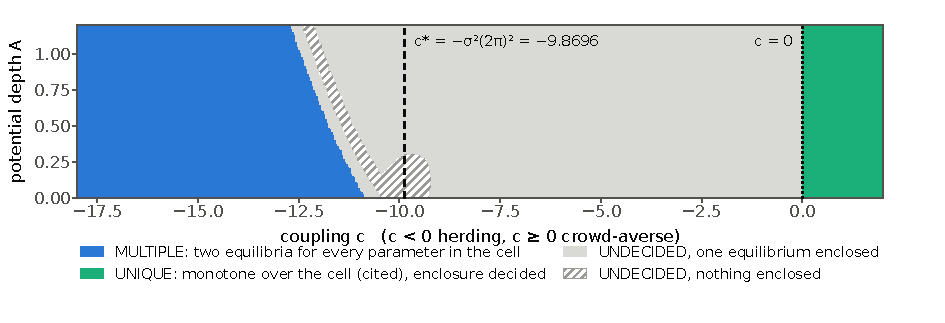
\includegraphics[width=\linewidth]{mfg-multiplicity-map1.pdf}
\caption{The record \texttt{certs/mfg-regime-map.json}: the $(c,A)$ plane of \eqref{eq:mfg} at $\sigma=\OneSigma$, $N=\OneN$, $\nu=\OneNu$, rasterised at the finest cell used, $\OneFinestC\times\OneFinestA$ ($\OneRasterC\times\OneRasterA$ pixels), each pixel taking the verdict of the cell covering it. Blue: \MULT\ (\OneMult\ cells); green: \UNIQ\ (\OneUniq); grey: \UNDEC\ with one solution enclosed (\OneUndEnclosed); hatched: \UNDEC\ with nothing enclosed (\OneUndNothing). Dashed: $\cstar=-\sigma^2(2\pi)^2$, where the linearisation of the constant state is singular and no enclosure can exist; the refusals there form the seam.}
\label{fig:map1}
\end{figure}

\begin{table}[!htb]\centering\footnotesize
\begin{tabular}{lrrr}\toprule
verdict & cells & area & share\\\midrule
\MULT & \OneMult & \OneMultArea & \OneMultPct\\
\UNIQ & \OneUniq & \OneUniqArea & \OneUniqPct\\
\UNDEC & \OneUnd & \OneUndArea & \OneUndPct\\
\quad one solution enclosed & \OneUndEnclosed & \OneUndEncArea & \OneUndEncPct\\\midrule
total & \OneCells & \OneDomainArea & \\
\bottomrule\end{tabular}
\qquad
\begin{tabular}{crrrrr}\toprule
depth & cell size ($c\times A$) & cells & \MULT & \UNIQ & \UNDEC\\\midrule
\OneDepthRows
\bottomrule\end{tabular}
\caption{The one-population map, $c\in[\OneCLo,\OneCHi]$, $A\in[\OneALo,\OneAHi]$, swept in \OneSeconds\ s on \OneGenerated. Above: the tally; the areas sum to the area of the rectangle. Below: the quadtree---a cell that refused for a repairable reason was quartered, to depth \OneMaxDepth, and the refined cells cluster on the seam at $\cstar$ and on the fold where the two branches meet.}
\label{tab:tally1}
\end{table}

\begin{table}[!htb]\centering\footnotesize
\begin{tabular}{rp{0.8\linewidth}}\toprule
cells & the reason, as the instrument stated it\\\midrule
\OneReasonRows
\bottomrule\end{tabular}
\caption{The \OneUnd\ undecided cells by reason. ``Only one solution found'' is the region above the fold, where the two branches have met: one solution is exhibited and nothing is said about its being alone. ``$Z_1\ge1$'' is a cell straddling a singular linearisation, the seam at $\cstar$.}
\label{tab:reasons1}
\end{table}

Table~\ref{tab:tally1} gives the tally and the quadtree, Table~\ref{tab:reasons1} the undecided reasons; the page that carries the map re-derives both at every build \cite{ObsPage}. The \MULT\ cells occupy $c\in[\OneMultCMin,\OneMultCMax]$, all of them below $\cstar$; the \UNIQ\ cells occupy $c\in[\OneUniqCMin,\OneUniqCMax]$. Over every \MULT\ cell the separation of the two predictors exceeds the sum of the two radii by a factor between \OneWorstSepRatio\ and \OneBestSepRatio; the largest radius is \OneMaxRadius, the largest contraction factor \OneWorstKappa, and the smallest certified density \OneMinDensity, in the cell $c\in\OneMinDensityC$, $A\in\OneMinDensityA$, where the herding density presses toward zero as the well deepens. The corridor $\cstar<c<0$ is undecided with one solution enclosed: the operator is not monotone there, the aligned branch is alone in this family, and the verdict is an enclosure without a uniqueness claim until $c$ reaches $0$.

\subsection{Two populations}

\begin{figure}[!htb]\centering
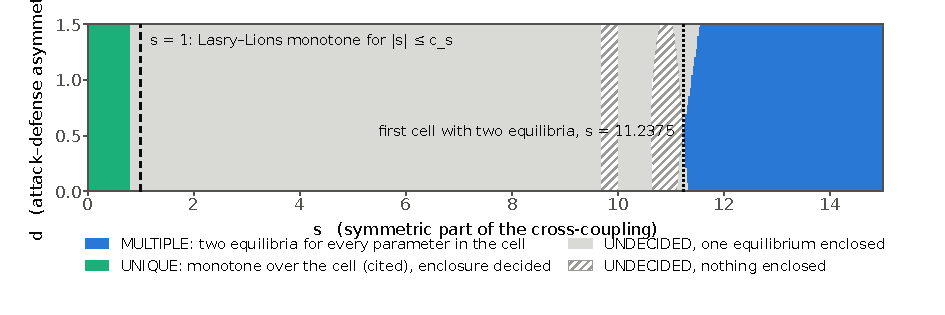
\includegraphics[width=\linewidth]{mfg-multiplicity-map2.pdf}
\caption{The record \texttt{certs/mfg2p-regime-map.json}: the $(s,d)$ plane of \eqref{eq:mfg2} at $\sigma=\TwoSigma$, $c_{11}=c_{22}=\TwoCs$, $A_1=A_2=\TwoA$, $N=\TwoN$, $\nu=\TwoNu$, rasterised at $\TwoFinestS\times\TwoFinestD$ ($\TwoRasterS\times\TwoRasterD$ pixels). Blue: \MULT\ (\TwoMult); green: \UNIQ\ (\TwoUniq); grey: \UNDEC\ with one equilibrium enclosed (\TwoUndEnclosed); hatched: \UNDEC\ with nothing enclosed (\TwoUndNothing). Dashed: $s=\TwoCs$, the Lasry--Lions boundary $|s|\le c_s$ on this slice; dotted: $s=\TwoMultSmin$, the first cell carrying two equilibria.}
\label{fig:map2}
\end{figure}

\begin{table}[!htb]\centering\footnotesize
\begin{tabular}{lrrr}\toprule
verdict & cells & area & share\\\midrule
\MULT & \TwoMult & \TwoMultArea & \TwoMultPct\\
\UNIQ & \TwoUniq & \TwoUniqArea & \TwoUniqPct\\
\UNDEC & \TwoUnd & \TwoUndArea & \TwoUndPct\\\midrule
total & \TwoCells & \TwoDomainArea & \\
\bottomrule\end{tabular}
\qquad
\begin{tabular}{lr}\toprule
cell size ($s\times d$) & cells\\\midrule
\TwoSizeRows
\bottomrule\end{tabular}
\qquad
\begin{tabular}{rp{0.36\linewidth}}\toprule
cells & reason\\\midrule
\TwoReasonRows
\bottomrule\end{tabular}
\caption{The two-population map, $s\in[\TwoSLo,\TwoSHi]$, $d\in[\TwoDLo,\TwoDHi]$ (record committed \TwoCommitDate). Top left: the tally. Top right: the cells by size, the two bands of the sweep and their one level of refinement. Below: the \TwoUnd\ undecided cells by reason; of the \TwoWhyMonotone\ in the first row, \TwoWhyMonotoneRef\ also held a second candidate whose certificate refused and sit at the depth limit.}
\label{tab:tally2}
\end{table}

Three readings of Figure~\ref{fig:map2} are supported by the record. The monotone region is decided as such only up to $s=\TwoUniqSmax$: a cell in $(s,d)$ is certified through the enclosing rectangle of its image in $(c_{12},c_{21})$, a strict superset, and the worst-corner test of $C+C^{\mathsf T}\succeq0$ fails on that superset for the cells touching $s=\TwoCs$; the \UNIQ\ cells carry a determinant lower bound of at least \TwoUniqDetMin, radii at most \TwoUniqRMax\ and densities at least \TwoUniqMinM. The first \MULT\ cell sits at $s\in\TwoFirstS$, $d\in\TwoFirstD$, a factor \TwoGap\ beyond the boundary of the cited condition; between the two lies a corridor of \TwoWhyMonotone\ cells in which one equilibrium is enclosed and no theorem available to us excludes a second, and the hatched cells near $s\approx\BatTwoUoneS$ are where a branch's certificate refused close to the singular Jacobian of the pitchfork. And \TwoMultUnreach\ of the \TwoMult\ \MULT\ cells (\TwoMultUnreachPct, covering \TwoMultUnreachAreaPct\ of the rectangle) lie wholly at $d>0$, where the symmetry is broken throughout, the primary branch is smooth and the segregated branch is not connected to it; two equilibria are nonetheless decided there for every parameter. Whether $d$ bounds the multiplicity region is \emph{not} settled: the \MULT\ cells reach $d=\TwoMultDmax$, the top edge of the swept rectangle. The witnesses: separation over the combined radii between \TwoWorstSepRatio\ and \TwoBestSepRatio, largest contraction factor \TwoWorstKappa, smallest density \TwoMinDensity. The sweep's warm-start atlas held the segregated branch at \TwoAtlasSeg\ nodes; the page's build gate re-reaches that branch by a different path, from the pitchfork at $d=0$ and then up in $d$, and re-certifies the sampled cells: finding a branch is search, certifying it is proof.

\section{Single-cell and single-instance theorems}\label{sec:theorems}

\begin{theorem}[one cell]\label{thm:cell}
Let $\sigma=\OneSigma$ and let $S$ be the cell $c\in\OneTightC$, $A\in\OneTightA$ of the one-population map (depth \OneTightDepth). For every $(c,A)\in S$ the system \eqref{eq:mfg} with $V=A\cos2\pi x$ has two distinct real-analytic solutions $(u_1,m_1,\rho_1)$, $(u_2,m_2,\rho_2)$ in the even subspace, each the unique solution in a ball of $\lnu$ ($\nu=\OneNu$) of radius \OneTightRAligned\ about the aligned predictor and \OneTightRHerding\ about the herding predictor respectively, with $\min m_1,\min m_2\ge\OneTightMinM$. The balls are disjoint: the separation of the predictors over the cell is at least \OneTightSep\ against a radii sum of at most \OneTightRSum, a factor \OneTightRatio; the first cosine coefficients of the two densities lie in $\OneTightBoneAligned$ and $\OneTightBoneHerding$.
\end{theorem}

\begin{proof}
Two box certificates over $S$: on the aligned branch $Y_0=$ \OneTightYzeroAligned, $Z_1=\OneTightZoneAligned$, $Z_2=\OneTightZtwoAligned$, $\kappa=\OneTightKappaAligned$; on the herding branch $Y_0=$ \OneTightYzeroHerding, $Z_1=\OneTightZoneHerding$, $Z_2=\OneTightZtwoHerding$, $\kappa=\OneTightKappaHerding$; Theorem~\ref{thm:uniform} and Definition~\ref{def:verdict}. The cell is the one with the smallest separation-to-radii ratio in the record, chosen as the hardest case; its numbers are those the record stores, and \texttt{node reports/mfg-certify.js} re-derives them from the cell alone.
\end{proof}

\begin{theorem}[the one-population map]\label{thm:map1}
For every $(c,A)$ in the union of the \OneMult\ \MULT\ cells of Figure~\ref{fig:map1}, a set of area \OneMultArea\ in a rectangle of area \OneDomainArea, the system \eqref{eq:mfg} at $\sigma=\OneSigma$ has at least two distinct real-analytic solutions with positive density. For every $(c,A)$ in the union of the \OneUniq\ \UNIQ\ cells the unique solution \cite{LL07} is enclosed in a ball of the stated radius; and in \OneUndEnclosed\ further cells a solution is enclosed.
\end{theorem}

\begin{theorem}[the two-population map]\label{thm:map2}
For every $(s,d)$ in the union of the \TwoMult\ \MULT\ cells of Figure~\ref{fig:map2}, the system \eqref{eq:mfg2} with $\sigma=\TwoSigma$, $c_{11}=c_{22}=\TwoCs$, $c_{12}=s+d$, $c_{21}=s-d$, $V_i=\TwoA\cos2\pi x$ has at least two distinct real-analytic solutions with both densities positive; the same holds at $(s,-d)$ by the population swap. For every $(s,d)$ in the \TwoUniq\ \UNIQ\ cells the coupling matrix is Lasry--Lions monotone and the unique solution is enclosed.
\end{theorem}

\begin{proof}[Proof of Theorems~\ref{thm:map1} and~\ref{thm:map2}]
Each cell of the records carries its own certificate; the tool that wrote the macros of this paper re-checks, cell by cell, that every \MULT\ cell has separation above the radii sum, both contraction factors below one and a positive density floor, that every \UNIQ\ cell satisfies the monotonicity test and carries an enclosure, and that the cells tile the rectangle, and it refuses to write a number otherwise.
\end{proof}

\begin{theorem}[at least three solutions]\label{thm:three}
Let $\sigma=\MultSigma$, $V\equiv0$, $\nu=\MultNu$. For each of the couplings $c=$ \MultCouplingsText\ the system \eqref{eq:mfg} has at least three distinct solutions: the constant state $(0,1,c)$, a symmetry-broken solution, and its image under the half-shift $x\mapsto x+\tfrac12$, each the unique solution in an $\lnu$ ball about its candidate, the three balls pairwise disjoint, with positive densities (Table~\ref{tab:three}); at $c=\MultBoundaryC$, inside the monotone regime, the continued branch collapses onto the constant state and nothing is claimed.
\end{theorem}

\begin{table}[!htb]\centering\footnotesize
\begin{tabular}{rrrrrrrr}\toprule
$c$ & $N$ & $r$ (constant) & $r$ (branch) & $\max\kappa$ & min distance & max radii sum & $\min m$ (branch)\\\midrule
\MultRows
\bottomrule\end{tabular}
\caption{The three disjoint uniqueness balls at each coupling (\texttt{certs/mfg-cap-multiplicity.json}, \MultDate). The mirror's numbers equal the branch's to the digits shown. Distances are lower bounds, radii upper bounds; the smallest density floor over every ball is \MultMinM, at $c=\MultCMax$.}
\label{tab:three}
\end{table}

\begin{theorem}[exactly three Galerkin solutions]\label{thm:census}
For $N\in\{2,3,4,5\}$ the $N$-mode even Galerkin truncation of \eqref{eq:mfg} with $\sigma=\MultSigma$, $c=-12$, $V\equiv0$, with $2\pi$ carried as an interval, has exactly three solutions in the box $B_N\subset\mathbb{R}^{2N+1}$ printed in the record: every sub-box of $B_N$ not containing one of them is eliminated by an interval residual or a Krawczyk exclusion, and each of the three is isolated by a Krawczyk box $K(X)\subset\operatorname{int}X$ \cite{Kr69,Mo77,Ru10}, so that it exists and is unique there. The three correspond one-to-one to the candidates of Theorem~\ref{thm:three}. The exhaustion at $N=5$ processed \CensusBoxesFive\ boxes in \CensusSecondsFive\ minutes, with the split off-centre (fraction \CensusSplit) because a midpoint split parks the constant solution on child boundaries indefinitely; the claim is about the truncation on $B_N$, and the count of solutions of the system itself is open (records \texttt{certs/mfg-cap-census-N\{2..5\}-c-12.json}, \CensusDate).
\end{theorem}

\begin{proposition}[the uniqueness wall]\label{prop:wall}
At $\sigma=\OneSigma$, $A=0$, the linearisation of the constant state is singular at $\cstar=\OneCStarSix$: the determinant of the Galerkin Jacobian changes sign across it (battery check B1 of the lifted kernel, $\cstar=\CapBoneCStar$), and no box certificate can exist on a cell straddling it; the instrument refuses there with $Z_1\ge1$ (check X1), and the map shows the refusal as a seam. On the two-population slice, the certified monotone region ends at $s=\TwoUniqSmax$, the cited condition at $s=\TwoCs$, and the first certified multiplicity begins at $s=\TwoMultSmin$; the primary branch's Jacobian changes sign at $s\approx\BatTwoUoneS$ for $d=0$, a floating-point measurement.
\end{proposition}

\paragraph{The monotone flow.} Lasry and Lions read \eqref{eq:mfg} as the zero of one operator on the pair $(m,u)$, $\mathcal A(m,u)=(cm+V+\sigma u''-\tfrac12(u')^2,\,-\sigma m''-(mu')')$, paired in $L^2$; Almulla, Ferreira and Gomes compute stationary games by the flow $(\dot m,\dot u)=-\mathcal A(m,u)$, which contracts in $L^2$ because $\mathcal A$ is monotone \cite{AFG17,FGT25}. Two integrations by parts on the torus give, for any pair with $m>0$ and any direction $(\delta m,\delta u)$,
\begin{equation}\label{eq:form}
\langle D\mathcal A(m,u)(\delta m,\delta u),(\delta m,\delta u)\rangle_{L^2}=c\int\delta m^2+\int m\,(\delta u')^2 ,
\end{equation}
so the linearised operator is positive semidefinite exactly when $c\ge0$, the Lasry--Lions condition, decided by inspection; for $c<0$ the direction $\delta m=\cos2\pi x$, $\delta u=0$ gives $c/2$. The instrument assembles the interval Jacobian of the flow on the even Galerkin space of order $N$ from the rows of the lifted kernel and requires $c/2$ back at that direction on every instance, a check on the assembly. A gradient flow $\dot z=-G(z)^{-1}\nabla E(z)$ has at an equilibrium the Jacobian $-G^{-1}\operatorname{Hess}E$, similar to the symmetric $-G^{-1/2}\operatorname{Hess}E\,G^{-1/2}$, hence a real spectrum; a certified non-real eigenvalue excludes every $(G,E)$ near the equilibrium.

\begin{theorem}[not a gradient flow]\label{thm:mono}
At each of the instances \MonoDecidedIds\ of Table~\ref{tab:mono} let $x^*$ be the equilibrium of the Galerkin monotone flow of order $N$ enclosed in a Krawczyk box of radius at most \MonoGalerkinRMax, and let $J$ be the Jacobian of the flow there. Then $J$ has an eigenvalue $\mu$ with $\operatorname{Im}\mu$ enclosed away from zero, between \MonoImMin\ and \MonoImMax\ across the five instances (the per-instance enclosures are in the table). Consequently there is no Riemannian metric $G$ and function $E$ on a neighbourhood of $x^*$ in the Galerkin space for which the flow is $-G^{-1}\nabla E$. At the instances \MonoUndecidedIds\ every eigenvalue reached by inverse iteration is real to floating-point precision and nothing is claimed.
\end{theorem}

\begin{proof}
The eigenpair is enclosed by a Krawczyk step on the $2n+2$ real unknowns (real and imaginary parts of the eigenvector and of $\mu$, the phase fixed by one component), with the interval Jacobian taken over the equilibrium's box, from a float eigenpair obtained by complex inverse iteration shifted at the closed-form modes of the constant state; $\operatorname{Im}\mu$ comes back as an interval not containing zero. At $A=0$ the per-mode block $\bigl(\begin{smallmatrix}-c&\sigma\lambda\\-\sigma\lambda&-\lambda\end{smallmatrix}\bigr)$, $\lambda=(2\pi k)^2$, has eigenvalues $\tfrac12\bigl(-(c+\lambda)\pm\sqrt{(c-\lambda)^2-4\sigma^2\lambda^2}\bigr)$, non-real exactly when $\lambda(1-2\sigma)<c<\lambda(1+2\sigma)$: the certified pair at C1 contains the mode-$1$ value $\MonoCOneClosedRe+\MonoCOneClosedIm\,i$; for $\sigma=0.3$, $c=2$ the mode-$1$ window is $(\MonoROneWindowLo,\MonoROneWindowHi)$, which is why R1 returns a real spectrum and is left undecided, and at H0 the closed form is real with one positive eigenvalue, \MonoHZeroPositive. The record \texttt{certs/monoflow-spectrum.json} is re-derived under a second by its battery (\MonoChecks\ checks, \MonoReds\ red controls, among them a symmetric matrix handed a complex shift, which must yield no non-real pair) \cite{MonoPage}.
\end{proof}

\begin{table}[!htb]\centering\scriptsize\setlength{\tabcolsep}{3pt}
\begin{tabular}{llllllrr}\toprule
id & $(\sigma,c,A)$ & branch & $N$ & verdict & $\mu$ enclosed, or what was reached & $r$ (Galerkin) & $r$ (PDE)\\\midrule
\MonoRows
\bottomrule\end{tabular}
\caption{The seven instances. The Galerkin radius is that of the Krawczyk box of the equilibrium; the PDE radius is the enclosure of the same candidate as a solution of \eqref{eq:mfg} by the lifted kernel, reported for scale and not used in the theorem. The form \eqref{eq:form} returned $c/2$ at $\delta m=\cos2\pi x$ on every instance.}
\label{tab:mono}
\end{table}

\section{Where certification stops: the frontier of the congestion certifier}\label{sec:frontier}

The same kind of certificate was applied, in the source laboratory from which the kernels of this repository were lifted, to the discounted congestion game of Gomes and Mitake \cite{GM15} with exponent $a=\tfrac12$,
\[
u-\sigma u''+\tfrac12(u')^2/\sqrt m=A\cos2\pi x+\gamma m,\qquad m-\sigma m''-(\sqrt m\,u')'=1,\qquad m>0,
\]
with $\gamma=\FrontierGamma$ and $\nu=\FrontierNu$. The one published point of that instrument, $(\sigma,A)=(\CongSigma,\CongA)$ at $N=\CongN$, encloses an equilibrium with radius \CongR, $Z_1=\CongZone$, $Z_2=\CongZtwo$, $Y_0=$ \CongYzero, $\min m\ge\CongMinM$ and $\min m^{-1/2}\ge\CongMinW$ over the whole ball, by a verifier in standard-library Python that travels inside the published page and that we re-ran for this document (\CongReds\ falsifiers fired) \cite{CongestPage}; the well-counting theorems of \cite{TerraPeaks} rest on the same instrument. Sweeping that certifier over the amplitude $A$ at six viscosities and four truncation orders measures where it stops certifying. The data were produced on \FrontierMeasured\ by a kernel identified by its hash (\FrontierKernelSha), are lifted into this repository with their hashes pinned, and are \emph{not} re-run here (the sweep took hours); \texttt{certs/frontier-measurement.json} re-derives every statement below from the pinned files and refuses if a pin has moved (\FrontierChecks\ checks, \FrontierReds\ red controls).

Two facts carry the section (Table~\ref{tab:ladders}). The boundary moves with the truncation: from $N=14$ to $N=40$ it rises by \FrontierRiseMin\ to \FrontierRiseMax\ percent at $\sigma\in\{\FrontierRiseSigmas\}$ and is still rising at the highest order run, so a boundary measured at one $N$ is a lower bound on the method's frontier, and a published $A^\star(\sigma)$ at fixed $N$ would be a resolution artefact at that level. One thing does not move: in the analytic tail of $Z_1$ every term but one carries a denominator growing with $N$; the exception is the reciprocal block's term, whose linear part has no derivative, and its coefficient is measured to be $N$-free. Since $Z_1$ dominates it, the amplitude $A_{\mathrm{rec}}(\sigma)$ at which it reaches one is a ceiling on certification at \emph{every} $N$, computable from the candidate alone; it came out bit-identical across the four orders, and $A^\star(N)/A_{\mathrm{rec}}$ climbs from \FrontierRatioMin\ to \FrontierRatioMax\ without reaching one. Whether $A^\star(N)\to A_{\mathrm{rec}}$ is not established; nothing here bounds where solutions exist, the existence theorem of \cite{GM15} being untouched in the refused region. Certified continuation over a parameter set is the literature's method \cite{DLM07,GLP16}; what is drawn here is narrower, a refusal named and a ceiling read off the code path.

\begin{figure}[!htb]\centering
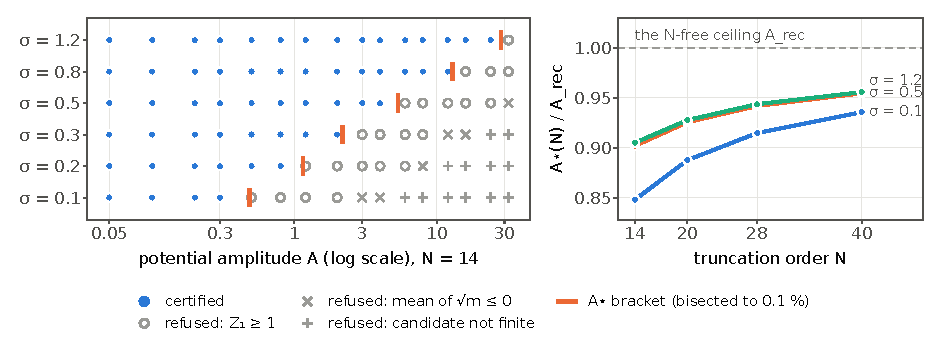
\includegraphics[width=\linewidth]{mfg-multiplicity-frontier.pdf}
\caption{Left: the six amplitude ladders at $N=14$ on a logarithmic axis, \FrontierGridCount\ amplitudes from \FrontierAMin\ to \FrontierAMax\ evaluated at every viscosity; every ladder is certified up to a boundary and refused beyond it, the first refusal always $Z_1\ge1$, the boundary bisected to a tenth of a percent (orange). Right: the certified boundary relative to the $N$-free ceiling $A_{\mathrm{rec}}$ rises with the truncation order at every viscosity and stays below one; the lines join decided brackets and are a trend, not a law.}
\label{fig:frontier}
\end{figure}

\begin{table}[!htb]\centering\scriptsize
\begin{tabular}{lrlrlrr}\toprule
$\sigma$ & $N$ & pattern & certified & $A^\star$ bracket & first refused $Z_1$ & $\min m$, last certified\\\midrule
\FrontierLadderRows
\bottomrule\end{tabular}
\\[6pt]
\begin{tabular}{lrrrrr}\toprule
$\sigma$ & $A^\star(14)$ & $A^\star(20)$ & $A^\star(28)$ & $A^\star(40)$ & rise\\\midrule
\FrontierRiseRows
\bottomrule\end{tabular}
\qquad
\begin{tabular}{llrrrr}\toprule
$\sigma$ & $A_{\mathrm{rec}}$ & $14$ & $20$ & $28$ & $40$\\\midrule
\FrontierCeilingRows
\bottomrule\end{tabular}
\caption{Top: the ladders; C is a certified point ($Z_1<1$, a radius, a positive density), R a refusal with a named mode, every pattern monotone; the first refusal on every ladder is $Z_1\ge1$, and the modes further out (a non-positive mean of $\sqrt m$, a non-finite candidate) are the solver's, not the certificate's. Middle: the lower end of the bisected bracket at four truncation orders, the candidate grid held at $1024$ points. Bottom: the $N$-free ceiling, bit-identical across $N$, and the ratio $A^\star(N)/A_{\mathrm{rec}}$ at each order.}
\label{tab:ladders}
\end{table}

\section{What is not claimed}\label{sec:notclaimed}

\begin{itemize}\setlength{\itemsep}{1pt}
\item Uniqueness outside the \UNIQ\ cells (in the corridors $\cstar<c<0$ and $\TwoUniqSmax<s<\TwoMultSmin$ one equilibrium is enclosed and nothing excludes a second), or any count beyond ``at least two'' in a \MULT\ cell; Theorem~\ref{thm:census} counts solutions of Galerkin truncations in a box, and the count for \eqref{eq:mfg} itself at $c=-12$ is open.
\item Anything off the slices swept: both maps hold $\sigma=\tfrac12$ (the $\sigma$ axis is the expensive one for this construction of $A$), the second holds $c_{11}=c_{22}=\TwoCs$ and $A_1=A_2=\TwoA$; whether $d$ bounds the multiplicity region is not settled.
\item That the phenomenon or the methods are new: multiplicity past the monotone regime is known \cite{Ci15,CV17,BF19,CDFP19}; that forward--backward systems are not gradient flows is structure, not discovery, and Theorem~\ref{thm:mono} is finite-dimensional, at the Galerkin order recorded; the radii-polynomial argument, the Krawczyk operator and interval arithmetic are the literature's \cite{DLM07,vdBL15,Kr69,Mo77,Ru10,Tu11}, and only the uniform-over-a-cell variant with its predictor, the refutation mode and the partition are this laboratory's engineering.
\item Any statement about published numerical solvers (the two-population page discusses why a solver descending from a natural initialisation lands on the primary branch and cannot see the second equilibrium when $d\ne0$ \cite{TwoPopPage}; we have re-run nobody's code), and independent reproduction: the records are published and re-runnable, not peer-reviewed and not independently rerun.
\end{itemize}

\cmrepro{\begin{sloppypar}The records are \path{certs/mfg-regime-map.json} (\OneCells\ cells, swept \OneGenerated), \path{certs/mfg2p-regime-map.json} (\TwoCells\ cells, committed \TwoCommitDate), \path{certs/mfg-cap-multiplicity.json}, \path{certs/mfg-cap-census-N{2,3,4,5}-c-12.json}, \path{certs/monoflow-spectrum.json} and \path{certs/frontier-measurement.json} (code hashes \MonoProvenanceSha\ldots\ and \FrontierProvenanceSha\ldots; data pinned under \path{corpus/refusal-frontier/}). The instruments are \path{labs/mfg/} and \path{labs/mfg2p/} (box certifiers, sweeps, batteries, the census and the multiplicity script), \path{instruments/monoflow/} and \path{instruments/frontier/}; the lifted point kernel is \path{legacy/core/mfg/}, with its hashes in \path{PROVENANCE.json}. One cell of the first map is re-decided from the cell alone by \texttt{node}~\path{reports/mfg-certify.js}~\texttt{'\{"sigma":0.5,"c":[-16.03,-15.97],"A":[0.288,0.313]\}'}, a file with no dependencies; the two-population map has no single-file certifier and is re-decided through \path{labs/mfg2p/box2p.js}. The batteries, each under five seconds, are \path{battery.js} in \path{labs/mfg/}, \path{labs/mfg2p/}, \path{instruments/monoflow/} and \path{instruments/frontier/}, and \path{legacy/research/mfg-cap/tests/test-cap.js}, run with \texttt{node}; the maps are rebuilt by \texttt{node}~\path{labs/mfg/regime.js} (\OneSecondsMin\ minutes) and \texttt{node}~\path{labs/mfg2p/regime2p.js}, the census by \texttt{node}~\path{labs/mfg/census.js}~\texttt{-{}-N 5 -{}-c -12} (\CensusSecondsFive\ minutes). The macros of this document are written by \texttt{node}~\path{tools/paper-numbers/mfg-multiplicity.js}, which re-runs the five batteries and the congestion verifier and refuses when a record no longer supports a sentence, and the figures by \path{tools/paper-numbers/mfg-multiplicity-figs.py}, from the records; repository commit \RepoCommit, pages at \url{https://carlostoledo.co/reports/}.\end{sloppypar}}

\begin{thebibliography}{99}\footnotesize\setlength{\itemsep}{0pt}
\bibitem{LL06a} J.-M. Lasry, P.-L. Lions, Jeux \`a champ moyen. I. Le cas stationnaire, C. R. Math. Acad. Sci. Paris 343 (2006) 619--625.
\bibitem{LL07} J.-M. Lasry, P.-L. Lions, Mean field games, Jpn. J. Math. 2 (2007) 229--260.
\bibitem{HMC06} M. Huang, R. P. Malham\'e, P. E. Caines, Large population stochastic dynamic games: closed-loop McKean--Vlasov systems and the Nash certainty equivalence principle, Commun. Inf. Syst. 6 (2006) 221--252.
\bibitem{BF19} M. Bardi, M. Fischer, On non-uniqueness and uniqueness of solutions in finite-horizon mean field games, ESAIM Control Optim. Calc. Var. 25 (2019), article 44.
\bibitem{Ci15} M. Cirant, Multi-population mean field games systems, J. Math. Pures Appl. 103 (2015) 1294--1315.
\bibitem{CV17} M. Cirant, G. Verzini, Bifurcation and segregation in quadratic two-populations mean field games systems, ESAIM Control Optim. Calc. Var. 23 (2017) 1145--1177; arXiv:1511.09343.
\bibitem{CDFP19} A. Cecchin, P. Dai Pra, M. Fischer, G. Pelino, On the convergence problem in mean field games: a two state model without uniqueness, SIAM J. Control Optim. 57 (2019) 2443--2466.
\bibitem{AFG17} N. Almulla, R. Ferreira, D. Gomes, Two numerical approaches to stationary mean-field games, Dyn. Games Appl. 7 (2017) 657--682, doi:10.1007/s13235-016-0203-5.
\bibitem{FGT25} R. Ferreira, D. Gomes, T. Tada, An introduction to monotonicity methods in mean-field games, arXiv:2502.20091 (2025).
\bibitem{GM15} D. A. Gomes, H. Mitake, Existence for stationary mean-field games with congestion and quadratic Hamiltonians, NoDEA Nonlinear Differential Equations Appl. 22 (2015) 1897--1910.
\bibitem{DLM07} S. Day, J.-P. Lessard, K. Mischaikow, Validated continuation for equilibria of PDEs, SIAM J. Numer. Anal. 45 (2007) 1398--1424.
\bibitem{vdBL15} J. B. van den Berg, J.-P. Lessard, Rigorous numerics in dynamics, Notices Amer. Math. Soc. 62 (2015) 1057--1061.
\bibitem{GLP16} M. Gameiro, J.-P. Lessard, A. Pugliese, Computation of smooth manifolds via rigorous multi-parameter continuation in infinite dimensions, Found. Comput. Math. 16 (2016) 531--575.
\bibitem{Kr69} R. Krawczyk, Newton-Algorithmen zur Bestimmung von Nullstellen mit Fehlerschranken, Computing 4 (1969) 187--201.
\bibitem{Mo77} R. E. Moore, A test for existence of solutions to nonlinear systems, SIAM J. Numer. Anal. 14 (1977) 611--615.
\bibitem{Ru10} S. M. Rump, Verification methods: rigorous results using floating-point arithmetic, Acta Numer. 19 (2010) 287--449.
\bibitem{Tu11} W. Tucker, Validated Numerics: A Short Introduction to Rigorous Computations, Princeton University Press, 2011.
\bibitem{TerraPeaks} C. Toledo, Gain-weighted well-counting in a congestion mean-field game, draft v0.2 (2026), \texttt{paper/terra-peaks.md} in the repository.
\bibitem{CapPage} C. Toledo, Two solutions, provably: certified multiplicity for a non-monotone MFG, \url{https://carlostoledo.co/reports/mfg-cap.html}; the kernel \texttt{legacy/core/mfg/} and its battery \texttt{legacy/research/mfg-cap/tests/test-cap.js}, lifted from the published \texttt{mfg-lab} tree.
\bibitem{ObsPage} C. Toledo, The MFG regime observatory, \url{https://carlostoledo.co/reports/mfg-observatory.html}.
\bibitem{TwoPopPage} C. Toledo, The attack--defense regime map, \url{https://carlostoledo.co/reports/mfg-two-population.html}.
\bibitem{CongestPage} C. Toledo, A congestion mean-field game, enclosed, \url{https://carlostoledo.co/reports/mfg-congest.html}; the frontier measurement, \url{https://carlostoledo.co/reports/frontier.html}.
\bibitem{MonoPage} C. Toledo, Monotone, and provably not a gradient, \url{https://carlostoledo.co/reports/monoflow.html}.
\end{thebibliography}

\end{document}
